%\documentclass[a4paper]{article}
%\usepackage[T1,T2A]{fontenc}
%\usepackage[utf8]{inputenc}
%\usepackage[english,russian]{babel}
%\usepackage{booktabs}
%\usepackage{color,colortbl}
%\usepackage{amsmath}
%\usepackage{amsfonts}
%\usepackage{amssymb}
%\usepackage{makeidx}
%\usepackage{tikz}
%\usetikzlibrary{graphs}
%\usepackage{graphicx}
%\definecolor{darkishgreen}{RGB}{39,203,22}
%\definecolor{LightCyan}{rgb}{0.88,1,1}
%\definecolor{Gray}{gray}{0.9}
%\definecolor{lightRed}{RGB}{230,170,150}
%\definecolor{modRed}{RGB}{230,82,90}
%\definecolor{strongRed}{RGB}{230,6,6}

%\usepackage[english,russian]{babel}

%\begin{document}

\section{Лабораторная работа №3.\newline Обработка данных в электронных таблицах}

Цель работы:
\begin{enumerate}
    \item Приобрести практические навыки по созданию и форматированию таблиц в MS Excel.
\end{enumerate}
\subsection{Теоретические основы}

Табличным процессором или электронной таблицей называется прикладная программа, предназначенная для хранения данных различных типов в табличной форме и их обработки. Табличные процессоры обеспечивают работу с большими таблицами чисел. При работе с табличным процессором на экран выводится прямоугольная таблица, в клетках которой могут находиться числа, пояснительные тексты и формулы для расчета значений в клетке по имеющимся данным. Особенность электронных таблиц заключается в возможности применения формул для описания связи между значениями различных ячеек. Расчет по заданным формулам выполняется автоматически. Изменение содержимого какой-либо ячейки приводит к пересчету значений всех ячеек, которые с ней связаны формульными отношениями и, тем самым, к обновлению всей таблицы в соответствии с изменившимися данными.

Применение электронных таблиц упрощает работу с данными и позволяет получать результаты без проведения расчетов вручную или специального программирования. Наиболее широкое применение электронные таблицы нашли в экономических и бухгалтерских расчетах, но и в научно-технических задачах электронные таблицы можно использовать эффективно, например для:

\begin{itemize}

  \item проведения однотипных расчетов над большими наборами данных
  \item автоматизации итоговых вычислений
  \item решения задач путем подбора значений параметров, табулирования формул
  \item обработки результатов экспериментов
  \item проведения поиска оптимальных значений параметров
  \item подготовки табличных документов
  \item построения диаграмм и графиков по имеющимся данным

\end{itemize}

Одним из наиболее распространенных средств работы с документами, имеющими табличную структуру, является программа Microsoft Excel.

Программа Microsoft Excel предназначена для работы с таблицами данных, преимущественно числовых. При формировании таблицы выполняют ввод, редактирование и форматирование текстовых и числовых данных, а также формул. Наличие средств автоматизации облегчает эти операции. Созданная таблица может быть выведена на печать.

\subsubsection{Рабочая книга и рабочий лист. Строки, столбцы, ячейки.}

Документ Excel называется рабочей книгой. Рабочая книга представляет собой набор рабочих листов, каждый из которых имеет табличную структуру и может содержать одну или несколько таблиц. В окне документа в программе Excel отображается только текущий рабочий лист, с которым и ведется работа. Каждый рабочий лист имеет название, которое отображается на ярлычке листа, отображаемом в его нижней части. С помощью ярлычков можно переключаться к другим рабочим листам, входящим в ту же самую рабочую книгу. Чтобы переименовать рабочий лист, надо дважды щелкнуть на его ярлычке. Рабочий лист состоит из строк и столбцов. Столбцы озаглавлены прописными латинскими буквами и, далее, двухбуквенными комбинациями. Всего рабочий лист может содержать до 256 столбцов, пронумерованных от А до IV. Строки последовательно нумеруются цифрами, от 1 до 65 536 (максимально допустимый номер строки).

\textbf{Ячейки и их адресация.} На пересечении столбцов и строк образуются ячейки таблицы. Они являются минимальными элементами для хранения данных. Обозначение отдельной ячейки сочетает в себе номера столбца и строки (в этом порядке), на пересечении которых она расположена, например: А1 или DE234. Обозначение ячейки (ее номер) выполняет функции ее адреса. Адреса ячеек используются при записи формул, определяющих взаимосвязь между значениями, расположенными в разных ячейках. Одна из ячеек всегда является активной и выделяется рамкой активной ячейки. Эта рамка в программе Excel играет роль курсора. Операции ввода и редактирования всегда производятся в активной ячейке. Переместить рамку активной ячейки можно с помощью курсорных клавиш или указателя мыши.

\textbf{Диапазон ячеек.} На данные, расположенные в соседних ячейках, можно ссылаться в формулах как на единое целое. Такую группу ячеек называют диапазоном. Наиболее часто используют прямоугольные диапазоны, образующиеся на пересечении группы последовательно идущих строк и группы последовательно идущих столбцов. Диапазон ячеек обозначают, указывая через двоеточие номера ячеек, расположенных в противоположных углах прямоугольника, например: А1 :С15. Если требуется выделить прямоугольный диапазон ячеек, это можно сделать протягиванием указателя от одной угловой ячейки до противоположной по диагонали. Рамка текущей ячейки при этом расширяется, охватывая весь выбранный диапазон. Чтобы выбрать столбец или строку целиком, следует щелкнуть на заголовке столбца (строки). Протягиванием указателя по заголовкам можно выбрать несколько идущих подряд столбцов или строк. Отдельная ячейка может содержать данные, относящиеся к одному из трех типов: текст, число или формула, --- а также оставаться пустой. Программа Excel при сохранении рабочей книги записывает в файл только прямоугольную область рабочих листов, примыкающую к левому верхнему углу (ячейка А1) и содержащую все заполненные ячейки. Тип данных, размещаемых в ячейке, определяется автоматически при вводе. Если эти данные можно интерпретировать как число, программа Excel так и делает. В противном случае данные рассматриваются как текст. Ввод формулы всегда начинается с символа «=» (знака равенства).

\subsubsection{Содержание электронной таблицы}

\textbf{Формулы.} Вычисления в таблицах программы Excel осуществляются при помощи формул. Формула может содержать числовые константы, ссылки на ячейки и функции Excel, соединенные знаками математических операций. Скобки позволяют изменять стандартный порядок выполнения действий. Если ячейка содержит формулу, то в рабочем листе отображается текущий результат вычисления этой формулы. Если сделать ячейку текущей, то сама формула отображается в строке формул.

\textbf{Ссылки на ячейки.} Формула может содержать ссылки, то есть адреса ячеек, содержимое которых используется в вычислениях. Это означает, что результат вычисления формулы зависит от числа, находящегося в другой ячейке. Ячейка, содержащая формулу, таким образом, является зависимой. Значение, отображаемое в ячейке с формулой, пересчитывается при изменении значения ячейки, на которую указывает ссылка. Ссылку на ячейку можно задать разными способами. Во-первых, адрес ячейки можно ввести вручную. Другой способ состоит в щелчке на нужной ячейке или выборе диапазона, адрес которого требуется ввести. Ячейка или диапазон при этом выделяются пунктирной рамкой. Все диалоговые окна программы Excel, которые требуют указания номеров или диапазонов ячеек, содержат кнопки, присоединенные к соответствующим полям. При щелчке на такой кнопке диалоговое окно сворачивается до минимально возможного размера, что облегчает выбор нужной ячейки (диапазона) с помощью щелчка или протягивания.

\textbf{Абсолютные и относительные ссылки.} По умолчанию, ссылки на ячейки в формулах рассматриваются как относительные. Это означает, что при копировании формулы адреса в ссылках автоматически изменяются в соответствии с относительным расположением исходной ячейки и создаваемой копии. Пусть, например, в ячейке В2 имеется ссылка на ячейку A3. В относительном представлении можно сказать, что ссылка указывает на ячейку, которая располагается на один столбец левее и на одну строку ниже данной. Если формула будет скопирована в другую ячейку, то такое относительное указание ссылки сохранится. Например, при копировании формулы в ячейку ЕА27 ссылка будет продолжать указывать на ячейку, располагающуюся левее и ниже, в данном случае на ячейку DZ28. При абсолютной адресации адреса ссылок при копировании не изменяются, так что ячейка, на которую указывает ссылка, рассматривается как нетабличная. Для изменения способа адресации при редактировании формулы надо выделить ссылку на ячейку и нажать клавишу F4. Элементы номера ячейки, использующие абсолютную адресацию, предваряются символом \$. Например, при последовательных нажатиях клавиши F4 номер ячейки А1 будет записываться как А1, \$А\$1, А\$1 и \$А1. В двух последних случаях один из компонентов номера ячейки рассматривается как абсолютный, а другой --- как относительный.

\newpage
\subsection{Задание на лабораторную работу}

Для выполнения работы необходимо:
\begin{enumerate}
  \item Изучить теоретический материал
  \item Выполнить все задания и сохранить в файле
  \item Оформить отчет по лабораторной работе
\end{enumerate}

\noindent\textbf{1. Заполните таблицу умножения используя формулы}

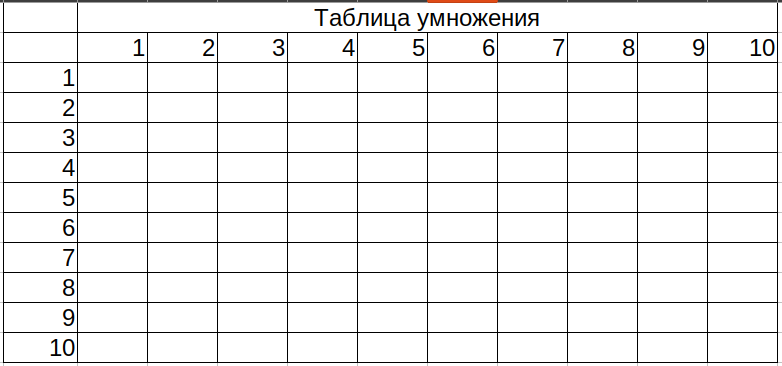
\includegraphics[width=\textwidth]{t1.png}

\noindent\textbf{2. Вычислить значения функции $y=\sin x$. Значения аргумента х изменяется от 0 до 10 с шагом 1. Постройте гладкий  график функции по таблице значений.}

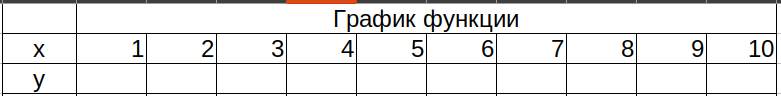
\includegraphics[width=\textwidth]{t2.png}

\noindent\textbf{3. Вычислить значения функции $x=16 * \sin^{3}t$ и $y = 13 * \cos(t) - 5 * \cos(2t) - 2 * \cos(3t) - \cos(4t)$. Значения аргумента x изменяется  от 0 до 6.4 с шагом 0.1. Постройте гладкий график функции по таблице значений}

\begin{center}
  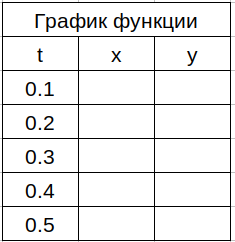
\includegraphics[width=120pt]{excel.png}
\end{center}
\newpage
\subsection{Содержание отчета}
\begin{enumerate}
  \item Титульный Лист
  \item Цель работы
  \item Краткие теоретические сведения по теме лабораторной работы
  \item Выполненное задание
  \item Краткий вывод о проделанной работе
\end{enumerate}

\begin{thebibliography}{3}
  \bibitem{iv1}
    Иванец, Г. Е. Табличный процессор MS Excel : учебное пособие / Г. Е. Иванец, Г. Е. Ивина. — Кемерово : Кемеровский технологический институт пищевой промышленности, 2007. — 107 c. — ISBN 978-5-89289-403-7. — Текст : электронный // Электронно-библиотечная система IPR BOOKS : [сайт]. — URL: http://www.iprbookshop.ru/14391.html
  \bibitem{bd2}
  Серогодский, В. В. Excel 2013 : пошаговый самоучитель + Справочник пользователя / В. В. Серогодский, А. Ю. Дружинин, Р. Г. Прокди. — Санкт-Петербург : Наука и Техника, 2014. — 400 c. — ISBN 978-5-94387-956-2. — Текст : электронный // Электронно-библиотечная система IPR BOOKS : [сайт]. — URL: http://www.iprbookshop.ru/35581.html
\end{thebibliography}


%\end{document}
